\documentclass[11pt]{article}

\usepackage{latexsym}
\usepackage{amssymb}
\usepackage{amsthm}
\usepackage{enumerate}
\usepackage{amsmath}
\usepackage{cancel}
\usepackage{graphicx}

\setlength{\evensidemargin}{.25in}
\setlength{\oddsidemargin}{-.25in}
\setlength{\topmargin}{-.75in}
\setlength{\textwidth}{6.5in}
\setlength{\textheight}{9.5in}
\newcommand{\due}{September 12th, 2012}
\newcommand{\HWnum}{1}
\input{/home/joey/Documents/Class/Define.tex}

\title{Notes on Measurement of Brownian Motion for Two SmA Islands}
\author{Joe Becker}

\begin{document}
\maketitle

We measured the relative Brownian motion of a Smectic A island interacting with another Smectic A island on a freely suspended film of 8CB liquid crystal. To achieve this we measure the relative motion of the islands parallel to the separation, $d$, and perpendicular to the separation, $\tau$. The geometry is shown in figure \ref{DTauFig}.

\begin{figure}
\centering
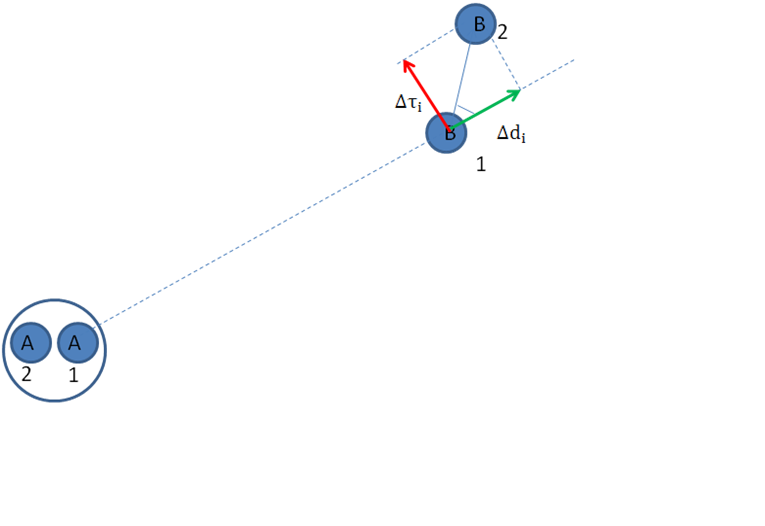
\includegraphics[scale=0.4]{Images/DTauFigure.png}
\caption{\textit{The geometry of $d$ and $\tau$.}}
\label{DTauFig}
\end{figure}

Note this operates under the assumption that the island A's movement is not large enough to affect the direction of $d$ and $\tau$. 

Note that the data collection is done through video of island motion through a $40\times$ objective. The video is decomposed into individual frames which allows the islands to be tracked. The tracking is done by an IDL algorithm written by Joe Maclennan which fits and ellipse to the islands and outputs the islands' center coordinates and the major and minor axes. A single tracked frame is shown in figure \ref{Tracked}.

\begin{figure}
\centering
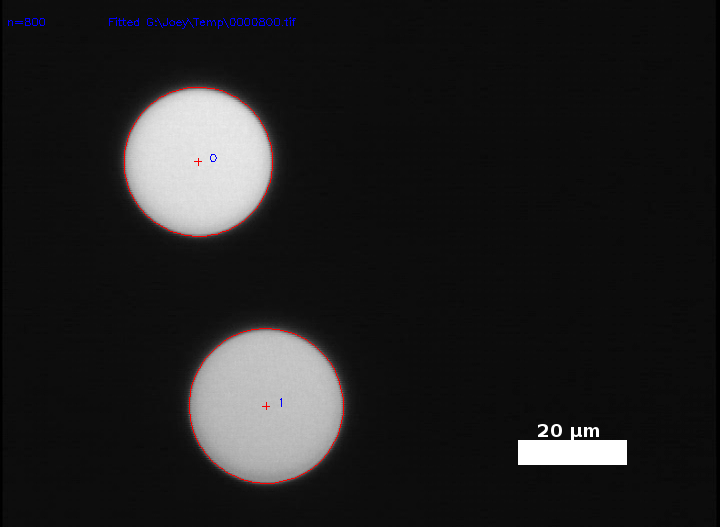
\includegraphics[scale=0.5]{Images/tracked.png}
\caption{\textit{An example tracking frame. The red ring is the ellipse fitted to the island.}}
\label{Tracked}
\end{figure}

From this tracking data we convert to the $d-\tau$ basis through the calculations
\begin{align}
d_n &= d_{n-1} + (x_{n}-x_{n-1})\cos(\theta_{n-1}) + (y_{n}-y_{n-1})\sin(\theta_{n-1})\\
\tau_n &= \tau_{n-1} + (y_{n}-y_{n-1})\cos(\theta_{n-1}) - (x_{n}-x_{n-1})\sin(\theta_{n-1})
\end{align}
where $\theta_n$ is the angle the separation line makes with the $x$ axis. It is calculated through the arctangent of the rectangular coordinates. We then analyze the tracked data by calculating the time step change of $d$ and $\tau$ over 8 to 12 time steps. This allows us to calculate the average change $\overline{\Delta d}_m$ and $\overline{\Delta\tau}_m$ for each timestep $m$. We then can find the variance from these means, $\sigma^{\tau}_m$ and $\sigma^{d}_m$. We obtain the diffusion constant by using the fact that the variance is proportional to elapsed time where the constant of proportionality is the diffusion constant. An example plot is shown in figure \ref{SigmaPlot}

\begin{figure}
\centering
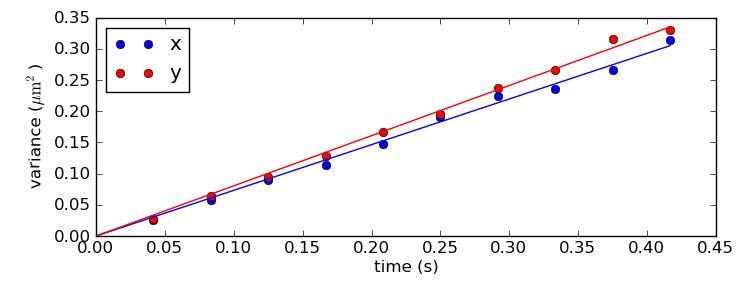
\includegraphics[scale=0.7]{Images/plot-001.png}
\caption{\textit{An example plot of $\sigma^{d}$ and $\sigma^{\tau}$ versus time. Note that the plot labeled $x$ corresponds to $d$ and the plot labeled $y$ corresponds to $\tau$.}}
\label{SigmaPlot}
\end{figure}

From here we wish to compare our measured results with the results generated by the model created by Tatiana. To do the we must convert our diffusion constant to a reduced mobility. This is done through the \emph{Einstein Relation}
\begin{equation}
D_T = k_BTb_T
\end{equation}
where $b$ is the mobility. We then find the reduced mobility by dividing out $\mu_0$ which is given by
$$\mu_0 = \frac{1}{4\pi\eta h}$$
where $\eta$ is the liquid crystal viscosity and $h$ is the film thickness. Note that the mobility is related to the reduced mobility, $\mu_T$, by
$$b_T = \mu_0\mu_T$$
So we calculate our reduced mobility by
$$\mu_T = \frac{D_T}{\mu_0k_BT} = \frac{4\pi\eta h}{k_BT}D_T$$.
Finally, we must account for the confinement which is not accounted for in the model. To do this we use Saffman's theory to get the reduced mobility due to the confinement effect as
$$\mu_{\textnormal{conf}} = \ln\left(\frac{R}{a}-\frac{1}{2}\right)$$
where $R$ is the radius of the film and $a$ is the radius of the island. We then correct the models prediction by 
$$\mu_{\textnormal{corr}} = \frac{\mu_{\textnormal{pred}}\mu_{\textnormal{conf}}}{\mu_{\textnormal{pred}}+\mu_{\textnormal{conf}}}$$
Figures \ref{RedMobd}, \ref{RedMobtau}, and \ref{ratio} show the comparison between the model and measured results.

\begin{figure}
\centering
\includegraphics[scale=0.4]{Images/2IslandRed.MobPerp.png}
\caption{\textit{Predicted and measured reduced mobility versus the ratio of separation and island radius. Note that this in the direction along the island separation.}}
\label{RedMobd}
\end{figure}

\begin{figure}
\centering
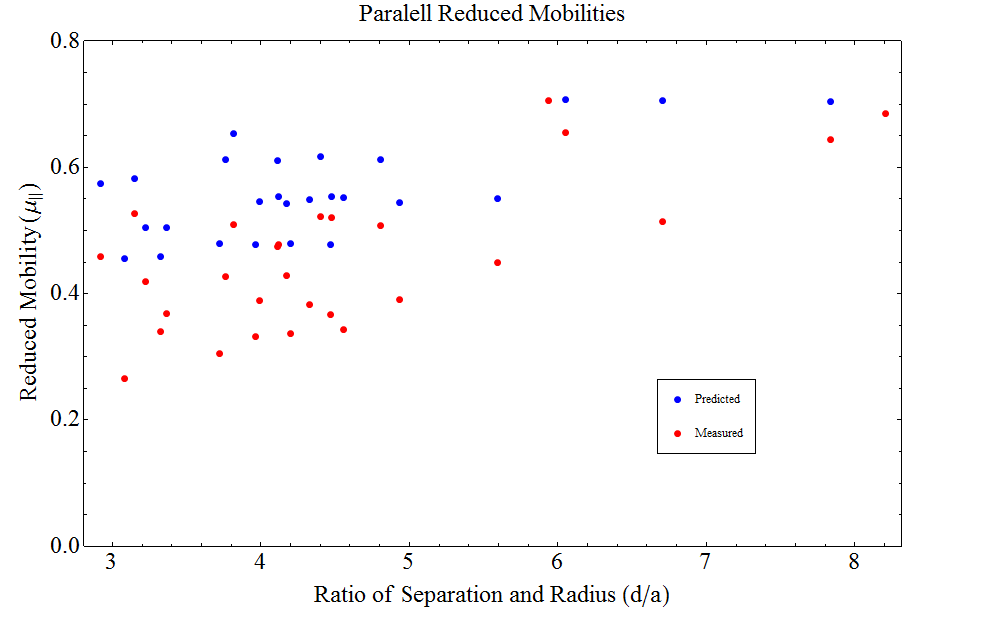
\includegraphics[scale=0.4]{Images/2IslandRedMobPara.png}
\caption{\textit{Predicted and measured reduced mobility versus the ratio of separation and island radius. Note that this in the direction perpendicular to the island separation.}}
\label{RedMobtau}
\end{figure}

\begin{figure}
\centering
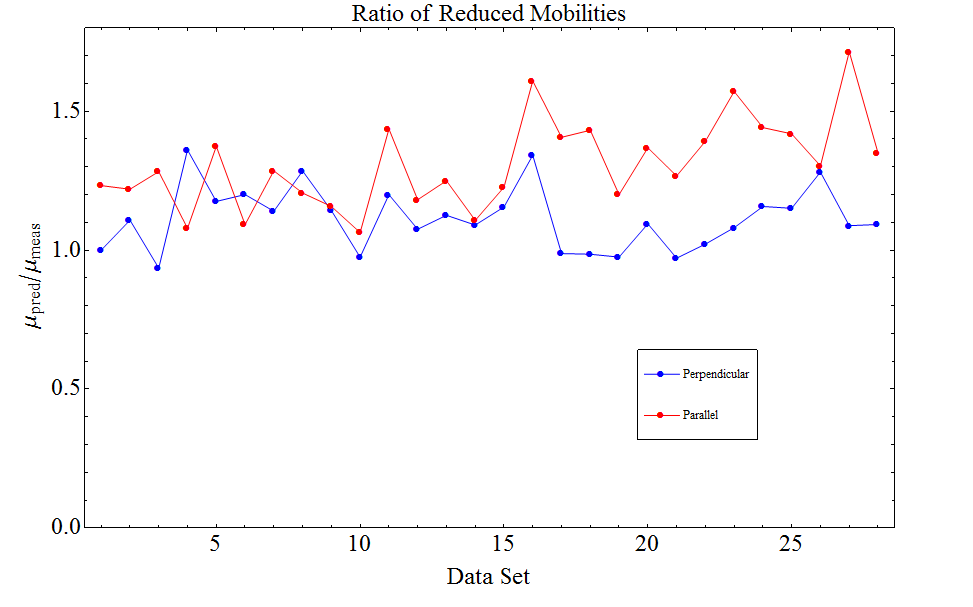
\includegraphics[scale=0.4]{Images/2IslandRedMobRatio.png}
\caption{\textit{Ratio of the reduced mobilities for both along and perpendicular to the island separation.}}
\label{ratio}
\end{figure}


\end{document}

